\section{Where to install batteries}\label{sec:storage}

We now solve the planning problem~\eqref{eq:siting} on the global panel.
For each commitment rule we take its out-of-sample hourly shortfalls and surpluses ($W=28$, eleven candidates with GFS and GEFS weather forecasts, decisions taken with the information available at the day-ahead gate closure), place a four-hour battery with 85\% round-trip efficiency in every grid area, and compute the annual value of battery power on a grid from 0 to 15\% of the area's mean demand.
Costs are converted to money by valuing one MWh of idle committed capacity at an illustrative \$10, so that a shortfall costs between \$40 and \$190 per MWh depending on the area's critical ratio; all dollar figures scale proportionally with this assumption.
The battery is dispatched greedily against the given commitment path, charging from committed-but-idle capacity and discharging into shortfalls; the commitment itself is not re-optimised with the battery in place, which would lower the commitment and the battery's value, especially for rules with large shortfalls.
The exercise values a single stream---cover for day-ahead commitment errors---and ignores arbitrage, adequacy, renewable firming and network deferral, which dominate real storage decisions.
It should be read as an illustration of how the operational rule changes the value and location of storage, conditional on this stream, not as a siting recommendation; and because the areas are observed over different periods, annual values are averages over each area's own evaluation period.

\subsection{Batteries do not pay for themselves on forecast errors alone}

The first increment of battery power is worth \$31,000--\$45,000 per MW-year in the median area of each continent (depending on the commitment rule), and at most \$73,000 (in the PJM interconnection).
Annualised costs of four-hour batteries are well above this range (we use \$100,000--\$200,000 per MW-year), so the cost-optimal battery size for covering day-ahead commitment errors alone is zero in every area and for every commitment rule.
Storage is deployed for arbitrage, capacity adequacy and the integration of renewables, and covering commitment errors is a by-product.
The relevant planning question is therefore not whether, but \emph{where}, to place the storage that energy-transition programmes already mandate, and how that choice depends on the way operators commit.

\subsection{Better commitment rules reduce the value of storage}

\begin{figure}[t]
\centering
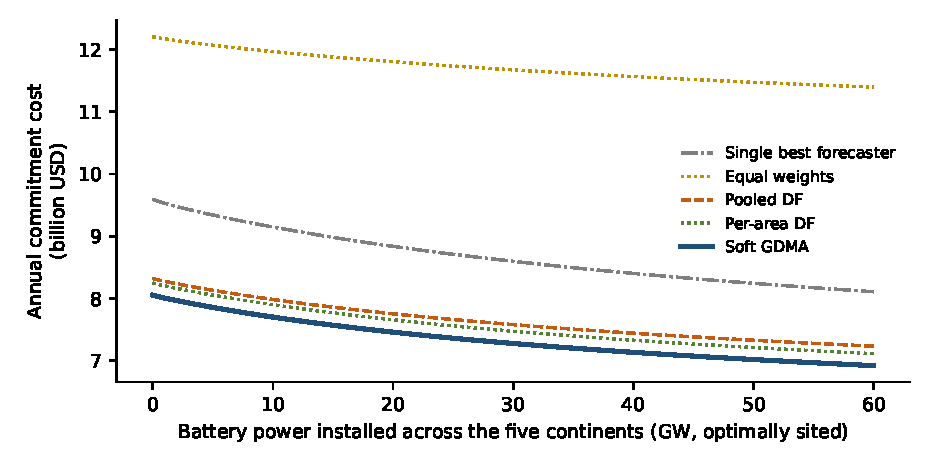
\includegraphics[width=0.9\textwidth]{figures/storage_frontier.pdf}
\caption{Annual system-wide commitment cost as a function of battery power installed and optimally sited across the 125 grid areas, for five commitment rules. Costs valued at \$10 per MWh of idle committed capacity; annual values average over each area's own evaluation period.}\label{fig:frontier}
\end{figure}

\begin{table}[t]
\centering
\caption{Storage siting on five continents. Cost of each commitment rule without storage, battery power it needs (optimally sited) to reach the cost of soft GDMA without storage, and the optimal siting of a 10\,GW storage programme.}\label{tab:storage}
\footnotesize
\setlength{\tabcolsep}{4pt}
\begin{tabular}{@{}lccccccc@{}}
\toprule
 & Cost without & GW to match & \multicolumn{5}{c}{Siting of a 10 GW budget (GW)} \\
\cmidrule(lr){4-8}
Commitment rule & storage (\$bn/yr) & soft GDMA$^c$ & N.\ Am. & Europe & Oceania & Asia & Africa \\
\midrule
Single best forecaster & 9.59 & $>60$ & 3.7 & 1.9 & 0.4 & 4.0 & 0.0 \\
Equal weights & 11.67 & $>60$ & 1.4 & 2.0 & 1.0 & 5.5 & 0.1 \\
Pooled DF & 8.25 & 7 & 2.1 & 2.4 & 0.5 & 5.0 & 0.0 \\
Per-area DF & 8.20 & 5 & 3.1 & 2.6 & 0.5 & 3.7 & 0.0 \\
Forecast-then-commit & 8.30 & 7 & 4.2 & 2.5 & 0.4 & 2.8 & 0.1 \\
GDMA & 8.05 & 1 & 2.5 & 2.5 & 0.5 & 4.4 & 0.1 \\
\textbf{Soft GDMA} & 8.00 & -- & 2.6 & 2.5 & 0.5 & 4.4 & 0.0 \\
\bottomrule
\end{tabular}
\par\smallskip\footnotesize $^c$ Smallest optimally sited budget, on a grid of 0.25\,GW steps up to 5\,GW and 1\,GW steps up to 60\,GW, at which the rule's cost falls to or below that of soft GDMA without storage.
\end{table}

Figure~\ref{fig:frontier} and Table~\ref{tab:storage} show how the operational rule and storage interact.
Without storage, soft GDMA commits the five continents' capacity for \$11.3 billion a year under the stylised cost model, against \$12.3 billion for the reference forecaster, a difference of \$1.0 billion or 8\%.
Adding batteries lowers every curve: the reference rule needs 34\,GW of optimally sited batteries to reach the cost that soft GDMA achieves without any, forecast-then-commit needs 17\,GW and per-area decision-focused weights 5\,GW, while pooled weights and plain GDMA are as cheap as soft GDMA without storage in this metric.
The battery-equivalent should not be read as the value of the better rule.
Batteries are credited here only with the commitment errors they absorb, so 34\,GW would cost far more than the \$1.0 billion difference in commitment cost; the relevant comparison for an operator is the direct saving.
The point is the interaction: the better the commitment rule, the less is left for storage to absorb, and a planner who values storage by today's errors overstates it.

\subsection{The siting decision depends on the commitment rule}

Table~\ref{tab:storage} also shows how a 10\,GW programme should be distributed.
Under soft GDMA, 4.3\,GW go to North America, 2.6\,GW to Europe, 0.7\,GW to Oceania and 2.5\,GW to Asia, and Africa receives almost nothing.
If the planner instead uses the error profile of the reference forecaster, North America receives 5.1\,GW, about 19\% more, because the U.S.\ balancing authorities' own forecasts leave the largest shortfalls; forecast-then-commit would send 5.0\,GW there.

\begin{table}[t]
\centering
\caption{Annual value (million USD) of storage programmes of different sizes when operations follow soft GDMA, by the commitment rule whose error profile was used to site the batteries.}\label{tab:siting}
\small
\begin{tabular}{@{}lcccc@{}}
\toprule
Siting based on & 1 GW & 5 GW & 10 GW & 20 GW \\
\midrule
Single best forecaster & 40 & 182 & 343 & 583 \\
Per-area DF & 45 & 194 & 351 & 593 \\
Forecast-then-commit & 40 & 186 & 344 & 588 \\
\textbf{Soft GDMA} & 47 & 197 & 353 & 594 \\
\bottomrule
\end{tabular}
\end{table}

Table~\ref{tab:siting} quantifies the cost of siting on the wrong profile, and it is modest: when operations follow soft GDMA, a 1\,GW programme sited with the reference rule's error profile delivers \$43 million a year instead of \$45 million, a 4\% loss; the loss is 4\% at 5\,GW, 3\% at 10\,GW and 2\% at 20\,GW.
The location of storage therefore matters less than the existence of a good commitment rule, but it is not irrelevant: the difference is a few per cent of the value of the programme, concentrated in North America.

\begin{table}[t]
\centering
\caption{Out-of-sample siting under soft GDMA operations (million USD per year): batteries are sited on the value curves of the first half of the evaluation period and valued on the second half, and compared with siting on the second half itself (infeasible oracle).}\label{tab:oos}
\small
\begin{tabular}{@{}lccc@{}}
\toprule
Budget & Sited on soft GDMA & Sited on the reference & Sited on the second \\
(GW) & (first half) & (first half) & half itself (oracle) \\
\midrule
1 & 44 & 42 & 47 \\
5 & 148 & 145 & 194 \\
10 & 247 & 232 & 336 \\
20 & 391 & 360 & 539 \\
\bottomrule
\end{tabular}
\end{table}

Siting on estimated value curves also carries estimation risk.
Table~\ref{tab:oos} sites batteries using the first half of the evaluation period and values them on the second half: siting on soft GDMA's own error profile captures about three quarters of the value of the infeasible oracle at 10\,GW (\$247 million of \$336 million), and siting on the reference rule's profile captures 6\% less than that at 10\,GW and 8\% less at 20\,GW.
Both sources of loss, the choice of rule and the estimation of the profile, are of similar size for programmes of 5--10\,GW, and the former does not dominate.

\subsection{Fair siting}

\begin{table}[t]
\centering
\caption{Efficient and fair siting of storage programmes under soft GDMA operations: annual value, the relative benefit of the worst-served continent, and the price of fairness (PoF, the share of the efficient programme's value given up).}\label{tab:fairsiting}
\footnotesize
\setlength{\tabcolsep}{4pt}
\begin{tabular}{@{}lccccccccc@{}}
\toprule
 & \multicolumn{2}{c}{Efficient} & \multicolumn{3}{c}{Proportional floors ($\lambda=1$)} & \multicolumn{3}{c}{Maximin} \\
\cmidrule(lr){2-3}\cmidrule(lr){4-6}\cmidrule(lr){7-9}
Budget & Value & Min.\ rel. & Value & Min.\ rel. & PoF & Value & Min.\ rel. & PoF \\
 (GW) & (\$m/yr) & benefit$^f$ & (\$m/yr) & benefit & & (\$m/yr) & benefit & \\
\midrule
1 & 45 & 0.0\% & 42 & 0.2\% & 7.3\% & 41 & 0.3\% & 9.0\% \\
5 & 191 & 0.6\% & 181 & 0.9\% & 5.0\% & 178 & 1.5\% & 6.9\% \\
10 & 338 & 1.4\% & 325 & 1.7\% & 3.9\% & 315 & 2.8\% & 7.0\% \\
20 & 571 & 3.1\% & 554 & 3.3\% & 3.0\% & 532 & 4.7\% & 6.7\% \\
\bottomrule
\end{tabular}
\par\smallskip\footnotesize $^f$ Lowest, across continents, of the value captured divided by the continent's annual commitment cost without storage.
\end{table}

Efficient siting concentrates batteries where the value in money is highest, and in small programmes some continents receive nothing: with 1\,GW, the worst-served continent's relative benefit is zero (Table~\ref{tab:fairsiting}).
Two fair rules respond differently.
Floors proportional to each continent's share of demand, the ``fair share'' rule often used in practice, raise the worst-served continent's relative benefit only slightly (from 1.4\% to 1.7\% of its commitment cost with 10\,GW) and give up 3--7\% of the programme's value.
Maximin siting, which directs every increment to the continent that has gained least so far, raises it much more---to 2.8\% with 10\,GW and from zero to 0.3\% with 1\,GW---at a price of fairness of 7--9\%.
Fairness in storage siting is therefore not free in this setting: protecting the worst-served continent costs between a thirtieth and a tenth of the programme's value, and a planner must decide whether that trade is worth making.
These figures condition on one value stream and on the continent as the unit of fairness; the within-continent distribution is not examined.
